\documentclass[]{article}
\usepackage{lmodern}
\usepackage{amssymb,amsmath}
\usepackage{ifxetex,ifluatex}
\usepackage{fixltx2e} % provides \textsubscript
\ifnum 0\ifxetex 1\fi\ifluatex 1\fi=0 % if pdftex
  \usepackage[T1]{fontenc}
  \usepackage[utf8]{inputenc}
\else % if luatex or xelatex
  \ifxetex
    \usepackage{mathspec}
  \else
    \usepackage{fontspec}
  \fi
  \defaultfontfeatures{Ligatures=TeX,Scale=MatchLowercase}
\fi
% use upquote if available, for straight quotes in verbatim environments
\IfFileExists{upquote.sty}{\usepackage{upquote}}{}
% use microtype if available
\IfFileExists{microtype.sty}{%
\usepackage{microtype}
\UseMicrotypeSet[protrusion]{basicmath} % disable protrusion for tt fonts
}{}
\usepackage[margin=1.3in]{geometry}
\usepackage{hyperref}
\hypersetup{unicode=true,
            pdftitle={Sistema de Colas},
            pdfauthor={\ldots{}.},
            pdfborder={0 0 0},
            breaklinks=true}
\urlstyle{same}  % don't use monospace font for urls
\usepackage{color}
\usepackage{fancyvrb}
\newcommand{\VerbBar}{|}
\newcommand{\VERB}{\Verb[commandchars=\\\{\}]}
\DefineVerbatimEnvironment{Highlighting}{Verbatim}{commandchars=\\\{\}}
% Add ',fontsize=\small' for more characters per line
\usepackage{framed}
\definecolor{shadecolor}{RGB}{248,248,248}
\newenvironment{Shaded}{\begin{snugshade}}{\end{snugshade}}
\newcommand{\KeywordTok}[1]{\textcolor[rgb]{0.13,0.29,0.53}{\textbf{#1}}}
\newcommand{\DataTypeTok}[1]{\textcolor[rgb]{0.13,0.29,0.53}{#1}}
\newcommand{\DecValTok}[1]{\textcolor[rgb]{0.00,0.00,0.81}{#1}}
\newcommand{\BaseNTok}[1]{\textcolor[rgb]{0.00,0.00,0.81}{#1}}
\newcommand{\FloatTok}[1]{\textcolor[rgb]{0.00,0.00,0.81}{#1}}
\newcommand{\ConstantTok}[1]{\textcolor[rgb]{0.00,0.00,0.00}{#1}}
\newcommand{\CharTok}[1]{\textcolor[rgb]{0.31,0.60,0.02}{#1}}
\newcommand{\SpecialCharTok}[1]{\textcolor[rgb]{0.00,0.00,0.00}{#1}}
\newcommand{\StringTok}[1]{\textcolor[rgb]{0.31,0.60,0.02}{#1}}
\newcommand{\VerbatimStringTok}[1]{\textcolor[rgb]{0.31,0.60,0.02}{#1}}
\newcommand{\SpecialStringTok}[1]{\textcolor[rgb]{0.31,0.60,0.02}{#1}}
\newcommand{\ImportTok}[1]{#1}
\newcommand{\CommentTok}[1]{\textcolor[rgb]{0.56,0.35,0.01}{\textit{#1}}}
\newcommand{\DocumentationTok}[1]{\textcolor[rgb]{0.56,0.35,0.01}{\textbf{\textit{#1}}}}
\newcommand{\AnnotationTok}[1]{\textcolor[rgb]{0.56,0.35,0.01}{\textbf{\textit{#1}}}}
\newcommand{\CommentVarTok}[1]{\textcolor[rgb]{0.56,0.35,0.01}{\textbf{\textit{#1}}}}
\newcommand{\OtherTok}[1]{\textcolor[rgb]{0.56,0.35,0.01}{#1}}
\newcommand{\FunctionTok}[1]{\textcolor[rgb]{0.00,0.00,0.00}{#1}}
\newcommand{\VariableTok}[1]{\textcolor[rgb]{0.00,0.00,0.00}{#1}}
\newcommand{\ControlFlowTok}[1]{\textcolor[rgb]{0.13,0.29,0.53}{\textbf{#1}}}
\newcommand{\OperatorTok}[1]{\textcolor[rgb]{0.81,0.36,0.00}{\textbf{#1}}}
\newcommand{\BuiltInTok}[1]{#1}
\newcommand{\ExtensionTok}[1]{#1}
\newcommand{\PreprocessorTok}[1]{\textcolor[rgb]{0.56,0.35,0.01}{\textit{#1}}}
\newcommand{\AttributeTok}[1]{\textcolor[rgb]{0.77,0.63,0.00}{#1}}
\newcommand{\RegionMarkerTok}[1]{#1}
\newcommand{\InformationTok}[1]{\textcolor[rgb]{0.56,0.35,0.01}{\textbf{\textit{#1}}}}
\newcommand{\WarningTok}[1]{\textcolor[rgb]{0.56,0.35,0.01}{\textbf{\textit{#1}}}}
\newcommand{\AlertTok}[1]{\textcolor[rgb]{0.94,0.16,0.16}{#1}}
\newcommand{\ErrorTok}[1]{\textcolor[rgb]{0.64,0.00,0.00}{\textbf{#1}}}
\newcommand{\NormalTok}[1]{#1}
\usepackage{graphicx,grffile}
\makeatletter
\def\maxwidth{\ifdim\Gin@nat@width>\linewidth\linewidth\else\Gin@nat@width\fi}
\def\maxheight{\ifdim\Gin@nat@height>\textheight\textheight\else\Gin@nat@height\fi}
\makeatother
% Scale images if necessary, so that they will not overflow the page
% margins by default, and it is still possible to overwrite the defaults
% using explicit options in \includegraphics[width, height, ...]{}
\setkeys{Gin}{width=\maxwidth,height=\maxheight,keepaspectratio}
\IfFileExists{parskip.sty}{%
\usepackage{parskip}
}{% else
\setlength{\parindent}{0pt}
\setlength{\parskip}{6pt plus 2pt minus 1pt}
}
\setlength{\emergencystretch}{3em}  % prevent overfull lines
\providecommand{\tightlist}{%
  \setlength{\itemsep}{0pt}\setlength{\parskip}{0pt}}
\setcounter{secnumdepth}{0}
% Redefines (sub)paragraphs to behave more like sections
\ifx\paragraph\undefined\else
\let\oldparagraph\paragraph
\renewcommand{\paragraph}[1]{\oldparagraph{#1}\mbox{}}
\fi
\ifx\subparagraph\undefined\else
\let\oldsubparagraph\subparagraph
\renewcommand{\subparagraph}[1]{\oldsubparagraph{#1}\mbox{}}
\fi

%%% Use protect on footnotes to avoid problems with footnotes in titles
\let\rmarkdownfootnote\footnote%
\def\footnote{\protect\rmarkdownfootnote}

%%% Change title format to be more compact
\usepackage{titling}

% Create subtitle command for use in maketitle
\providecommand{\subtitle}[1]{
  \posttitle{
    \begin{center}\large#1\end{center}
    }
}

\setlength{\droptitle}{-2em}

  \title{Sistema de Colas}
    \pretitle{\vspace{\droptitle}\centering\huge}
  \posttitle{\par}
    \author{\ldots{}.}
    \preauthor{\centering\large\emph}
  \postauthor{\par}
      \predate{\centering\large\emph}
  \postdate{\par}
    \date{Julio, 2019}

\usepackage{fancyhdr}
\pagestyle{fancy}
% ************* Encabezado y Pie de Pagina (Imagen) *****************
%\SetWatermarkText{
\includegraphics[width = .07\textwidth]{epn_logo.jpg}}
%\lhead{
\includegraphics[width = .08\textwidth]{epn_logo.jpg}}
\lfoot{
\includegraphics[width = .11\textwidth]{epn_logo.jpg}}
%\lfoot{
\includegraphics[width = .07\textwidth]{epn_logo2.png}}

\usepackage{titling}

\pretitle{%
  \begin{center}
  \LARGE
  
\includegraphics[width=4cm,height=6cm]{epn_logo2.png}\\[\bigskipamount]
}
\posttitle{\end{center}}

\begin{document}
\maketitle

\begin{verbatim}
## Warning: package 'knitr' was built under R version 3.6.1
\end{verbatim}

\clearpage
\tableofcontents
\clearpage

\section{Objetivos}\label{objetivos}

El principal objetivo de este trabajo es primero explicar como funciona
un sistema de colas, su importancia, y como modelar este proceso. Y el
segundo objetivo es estudiar y comparar el rendimiento de un sistema de
colas, utilizando dos modelos, el primero es el \textbf{G/G/K}, mientras
el otro supone una variante del mismo al asumir que el número \textbf{K}
de servidores es variable, y su dinámica depende de cierta política
preestablecida.

\section{Introducción}\label{introduccion}

Todos hemos experimentado en alguna ocasión la sensación de estar
perdiendo el tiempo al esperar en una cola. El fenómeno de las colas nos
parece natural: esperamos en el coche al estar en un tapón, o un
semáforo mal regulado, o en un peaje; esperamos en el teléfono a que nos
atienda un operador y en la cola de un supermercado para pagar. Pero a
veces las esperas son buenas. Nos hacen visualizar la importancia del
producto o servicio que vamos a adquirir, nos permiten pensar y
reconfigurar nuestro requerimiento. Pero en general como clientes no
queremos esperar, los gestores de los citados servicios no quieren que
esperemos. ¿Por qué hay que esperar? ¿Cuánto hay que esperar?. La
respuesta es casi siempre simple, en algún momento la capacidad de
servicio ha sido menor que la capacidad demandada. Esta limitación se
puede eliminar invirtiendo en elementos que aumenten la capacidad. En
estos casos la pregunta es: ¿Compensa invertir en máquinas, o mejor
invertimos en salas de espera?. La teoría de colas intenta responder a
estas preguntas utilizando la simulación como herramienta principal.

\section{Descripción de un sistema de
colas}\label{descripcion-de-un-sistema-de-colas}

Un sistema de colas se puede describir como sigue. Un conjunto de
``clientes'' llega a un sistema buscando un servicio, esperan si este no
es inmediato, y abandonan el sistema una vez han sido atendidos. El
término ``cliente'' se usa con un sentido general y no implica que sea
un ser humano, puede significar piezas esperando su turno para ser
procesadas o una lista de trabajo esperando para imprimir en una
impresora en red. La teoría de colas fue originariamente un trabajo
práctico. La primera aplicación de la que se tiene noticia es del
matemático danés Erlang sobre conversaciones telefónicas en 1909, para
el cálculo de tamaño de centralitas. Después se convirtió en un concepto
teórico que consiguió un gran desarrollo más aun en los últimos años, en
parte ayudado del desarrollo tecnológico reflejado en la potencia
computacional de nuestras actuales máquinas.

\section{Características de los sistemas de
colas}\label{caracteristicas-de-los-sistemas-de-colas}

Seis son las características básicas que se deben utilizar para
describir adecuadamente un sistema de colas:

\begin{itemize}
\tightlist
\item
  Patrón de llegada de los clientes
\item
  Patrón de servicio de los servidores
\item
  Disciplina de cola
\item
  Capacidad del sistema
\item
  Número de canales de servicio
\item
  Número de etapas de servicio
\end{itemize}

\section{Como medir el rendimiento de un
sistema}\label{como-medir-el-rendimiento-de-un-sistema}

La tarea de un analista de colas puede ser de dos tipo: primero
establecer mecanismos para medir la efectividad del sistema, o diseñar
un sistema ``óptimo'' (de acuerdo a algún criterio).

Diseñar eficientemente consiste, básicamente, en definir un sistema cuyo
coste de diseño y de operación se justifique por el servicio que da.
Dicho servicio se puede evaluar mediante el costo de ``no darlo''. De
este modo al diseñar se pretende minimizar unos supuestos costos
totales. A partir de los datos que nos suministra la teoría de colas se
puede obtener la información necesaria para definir el número de
asientos necesarios en una sala de espera, o la estructura de etapas de
un proceso de atención al cliente. En cualquier caso, para poder tomar
decisiones hacen falta datos que la teoría de colas puede dar en alguno
de los siguientes tres aspectos:

\begin{itemize}
\tightlist
\item
  tiempo de espera (en el total del sistema o en la cola)
\item
  cantidad de clientes esperando (en el sistema o en las colas)
\item
  tiempo ocioso de los servidores (total o particular de cada servicio)
\end{itemize}

\clearpage

\section{Sistema de colas G/G/K}\label{sistema-de-colas-ggk}

Un sistema con servidores en paralelo se caracteriza porque hay más de
un servidor que ejecuta la misma función con la misma eficiencia. Es un
sistema con \(k\) servidores en paralelo y donde no hay varias colas,
sino una sola.

Se asume que los tiempos de arribo de los clientes se distribuyen con
una función general, es decir \(t_a \sim D_1\), y además se tiene que
los tiempos de servicio de todos los servidores siguen una misma
distribución general digamos \(y \sim D_2\).

\subsection{Descripción de Parámetros}\label{descripcion-de-parametros}

\textbf{Variables de tiempo} \(t,T\)

\textbf{Variables de conteo}

\begin{itemize}
\tightlist
\item
  \(N_{A}\), número de llegadas hasta el tiempo t.
\item
  \(C_{j}\), número de clientes atendidos por el servidor
  \(j, j=1,2,...,k\), donde \textit{k} es el número de servidores
  abiertos hasta el instante \textit{t}.
\end{itemize}

\textbf{Variables de salida}

\begin{itemize}
\tightlist
\item
  \(A(n)\): la hora de llegada del cliente n, \(n\leq1\)
\item
  \(D(n)\): la hora de salida del cliente n, \(n\leq1\)
\end{itemize}

\textbf{Variables de estado} \[ ES=(n,i_{1},i_{2},...,i_{k}) \]

\begin{itemize}
\tightlist
\item
  \textit{n}: número de clientes en el sistema.
\item
  \(i_k\): i-ésimo cliente que va a estar en el servidor \textit{k}.
\end{itemize}

\textbf{Lista de eventos} \[LE=(t_a,tt,t_s)\]

\begin{itemize}
\tightlist
\item
  \(t_a\): hora del arribo.
\item
  \(tt\): hora de la atención.
\item
  \(t_s\): hora de la salida.
\end{itemize}

Con estas consideraciones, lo que nuestro código nos devuelve es una
lista con los siguientes datos:

\begin{itemize}
\tightlist
\item
  Tiempos de Arribo del n-ésimo cliente \(A(n)\)
\item
  Tiempos de Atención del n-ésimo cliente \(I(n)\)
\item
  Tiempos de Finalización del servicio del n-ésimo cliente \(D(n)\)
\item
  Cantidad de Clientes atendida por cada servidor \(C_j\).
\item
  Tiempo total que esperaron los clientes en la fila.
\item
  Tiempo total que estuvieron los servidores desocupados.
\end{itemize}

\subsection{Implementación}\label{implementacion}

Bajo estos supuestos hemos implementado en R un código para simular este
proceso, mismo que mostramos a continuación:

\begin{Shaded}
\begin{Highlighting}[]
\NormalTok{cola_ggk<-}\ControlFlowTok{function}\NormalTok{(}\DataTypeTok{T=}\DecValTok{50}\NormalTok{,}\DataTypeTok{lambda=}\DecValTok{10}\NormalTok{,}\DataTypeTok{mu=}\DecValTok{2}\NormalTok{,}\DataTypeTok{k=}\DecValTok{5}\NormalTok{)\{}
  \CommentTok{#+++++++++++++++ Funciones Extra +++++++++++++++++++}
  \CommentTok{#Funcion que genera tiempos de llegada }
\NormalTok{  gen_T<-}\ControlFlowTok{function}\NormalTok{(}\DataTypeTok{la=}\NormalTok{lambda)\{}\KeywordTok{rexp}\NormalTok{(}\DecValTok{1}\NormalTok{,la);\}}
  \CommentTok{#Funcion que genera tiempos de servicio}
\NormalTok{  gen_Y<-}\ControlFlowTok{function}\NormalTok{(}\DataTypeTok{muh=}\NormalTok{mu)\{}\KeywordTok{rexp}\NormalTok{(}\DecValTok{1}\NormalTok{,muh);\}}
  \CommentTok{#Funcion para Tiempo de Servicio Cliente}
\NormalTok{  tmp_clientes<-}\ControlFlowTok{function}\NormalTok{(I,A)\{}
\NormalTok{    s<-}\DecValTok{0}\NormalTok{;}
    \ControlFlowTok{for}\NormalTok{(i }\ControlFlowTok{in} \DecValTok{1}\OperatorTok{:}\KeywordTok{length}\NormalTok{(I))\{s<-s}\OperatorTok{+}\NormalTok{I[i]}\OperatorTok{-}\NormalTok{A[i];\}}
\NormalTok{    s<-s}\OperatorTok{/}\KeywordTok{length}\NormalTok{(I);}\KeywordTok{return}\NormalTok{(s);}
\NormalTok{  \}}
  \CommentTok{#++++++++++++  Inicializa Parámetros  +++++++++++++++}
\NormalTok{  t<-}\DecValTok{0}\NormalTok{;Na<-}\DecValTok{0}\NormalTok{;C<-}\KeywordTok{rep}\NormalTok{(}\DecValTok{0}\NormalTok{,k);t1<-}\KeywordTok{rep}\NormalTok{(}\DecValTok{0}\NormalTok{,k);}
\NormalTok{  tmuerto<-}\KeywordTok{rep}\NormalTok{(}\DecValTok{0}\NormalTok{,k);n<-}\DecValTok{0}\NormalTok{;i<-}\KeywordTok{rep}\NormalTok{(}\DecValTok{0}\NormalTok{,k);}
\NormalTok{  ta<-}\KeywordTok{rexp}\NormalTok{(}\DecValTok{1}\NormalTok{,lambda);tt<-}\KeywordTok{rep}\NormalTok{(}\OtherTok{Inf}\NormalTok{,k);}
  \CommentTok{#Variables de Salida}
\NormalTok{  A=}\OtherTok{NULL}\NormalTok{;I=}\OtherTok{NULL}\NormalTok{;D=}\OtherTok{NULL}\NormalTok{;}
  \CommentTok{#++++++++++++++++  Inicio  ++++++++++++++++++++++++}
  \ControlFlowTok{while}\NormalTok{(t}\OperatorTok{<=}\NormalTok{T)\{}
    \ControlFlowTok{if}\NormalTok{(ta}\OperatorTok{<}\KeywordTok{min}\NormalTok{(tt))\{}
\NormalTok{      t<-ta;Na<-Na}\OperatorTok{+}\DecValTok{1}\NormalTok{;ta<-ta}\OperatorTok{+}\KeywordTok{gen_T}\NormalTok{();}
\NormalTok{      A<-}\KeywordTok{c}\NormalTok{(A,t);a<-n;}
      \ControlFlowTok{if}\NormalTok{(n}\OperatorTok{<}\NormalTok{k)\{}
\NormalTok{        j<-}\DecValTok{1}\NormalTok{;}
        \ControlFlowTok{while}\NormalTok{(n}\OperatorTok{==}\NormalTok{a)\{}
          \ControlFlowTok{if}\NormalTok{(i[j]}\OperatorTok{==}\DecValTok{0}\NormalTok{)\{}
\NormalTok{            i[j]<-Na;tt[j]<-t}\OperatorTok{+}\KeywordTok{gen_Y}\NormalTok{();}
\NormalTok{            n<-n}\OperatorTok{+}\DecValTok{1}\NormalTok{;I[Na]<-t;}
\NormalTok{          \}}\ControlFlowTok{else}\NormalTok{\{}
\NormalTok{            j<-j}\OperatorTok{+}\DecValTok{1}\NormalTok{;}
\NormalTok{          \}}
\NormalTok{        \}}
\NormalTok{        tmuerto[j]<-tmuerto[j]}\OperatorTok{+}\NormalTok{(t}\OperatorTok{-}\NormalTok{t1[j]);}
\NormalTok{      \}}\ControlFlowTok{else}\NormalTok{\{}
\NormalTok{        n<-n}\OperatorTok{+}\DecValTok{1}\NormalTok{;}
\NormalTok{      \}}
\NormalTok{    \}}\ControlFlowTok{else}\NormalTok{\{}
\NormalTok{      ind<-}\KeywordTok{which.min}\NormalTok{(tt);t<-tt[ind];}
\NormalTok{      C[ind]<-C[ind]}\OperatorTok{+}\DecValTok{1}\NormalTok{;D[i[ind]]<-t;}
      \ControlFlowTok{if}\NormalTok{(n}\OperatorTok{<=}\NormalTok{k)\{}
\NormalTok{        i[ind]<-}\DecValTok{0}\NormalTok{;tt[ind]<-}\OtherTok{Inf}\NormalTok{;}
\NormalTok{        t1[ind]<-t;}
\NormalTok{      \}}\ControlFlowTok{else}\NormalTok{\{}
\NormalTok{        m<-}\KeywordTok{max}\NormalTok{(i);i[ind]<-m}\OperatorTok{+}\DecValTok{1}\NormalTok{;}
\NormalTok{        tt[ind]<-t}\OperatorTok{+}\KeywordTok{gen_Y}\NormalTok{();I[m}\OperatorTok{+}\DecValTok{1}\NormalTok{]<-t;}
\NormalTok{      \}}
\NormalTok{      n<-n}\OperatorTok{-}\DecValTok{1}\NormalTok{;       }
\NormalTok{    \}}
    
\NormalTok{  \}}
  \ControlFlowTok{while}\NormalTok{(n}\OperatorTok{>}\DecValTok{0}\NormalTok{)\{}
\NormalTok{    ind<-}\KeywordTok{which.min}\NormalTok{(tt);t<-tt[ind];}
\NormalTok{    C[ind]<-C[ind]}\OperatorTok{+}\DecValTok{1}\NormalTok{;D[i[ind]]<-t;}
    \ControlFlowTok{if}\NormalTok{(n}\OperatorTok{<=}\NormalTok{k)\{}
\NormalTok{      i[ind]<-}\DecValTok{0}\NormalTok{;tt[ind]<-}\OtherTok{Inf}\NormalTok{;}
\NormalTok{    \}}\ControlFlowTok{else}\NormalTok{\{}
\NormalTok{      m<-}\KeywordTok{max}\NormalTok{(i);i[ind]<-m}\OperatorTok{+}\DecValTok{1}\NormalTok{;}
\NormalTok{      tt[ind]<-t}\OperatorTok{+}\KeywordTok{gen_Y}\NormalTok{();I[m}\OperatorTok{+}\DecValTok{1}\NormalTok{]<-t;}
\NormalTok{    \}}
\NormalTok{    n<-n}\OperatorTok{-}\DecValTok{1}\NormalTok{;}
\NormalTok{  \}}

\NormalTok{  tmuertoserv<-}\KeywordTok{sum}\NormalTok{(tmuerto)}\OperatorTok{/}\KeywordTok{length}\NormalTok{(A);}
  
  \KeywordTok{return}\NormalTok{(}\KeywordTok{list}\NormalTok{(}\DataTypeTok{T_llegada=}\NormalTok{A,}\DataTypeTok{T_atendido=}\NormalTok{I,}\DataTypeTok{T_partida=}\NormalTok{D,}
            \DataTypeTok{Cantidad_atendida_x_servidores=}\NormalTok{C,}
            \DataTypeTok{T_muerto_cli=}\KeywordTok{tmp_clientes}\NormalTok{(I,A),}
            \DataTypeTok{T_muerto_serv=}\NormalTok{tmuertoserv));}
\NormalTok{\}}
\CommentTok{#+++++++++++++++++++  FIN +++++++++++++++++++++++++}
\end{Highlighting}
\end{Shaded}

A continuación ejecutamos la función que simula el sistema de colas
G/G/K, considerando un horizonte de tiempo \(T=10\) horas, y
distribuciones exponenciales de parámetros \(\lambda=10\), \(\mu=2\) y
considerando \(K=5\) el número de servidores activos.

Usaremos el paquete \texttt{ggplot2} para poder visualizar algunas de
las salidas de la función que simula el G/G/K, y obtenemos los
siguientes resultados:

\subsection{Gráficos}\label{graficos}

\begin{flushright}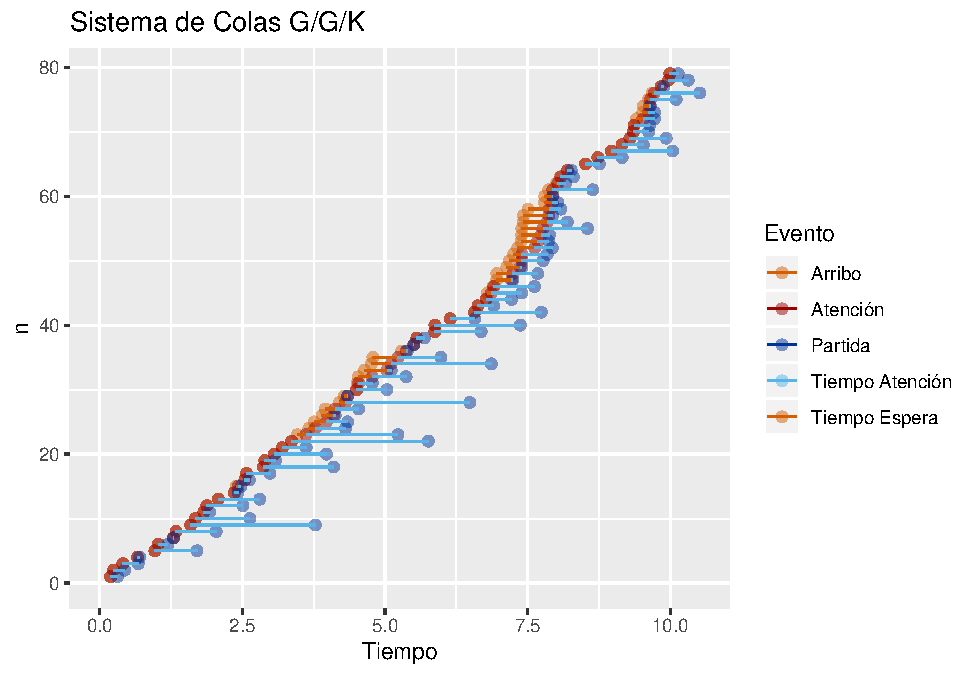
\includegraphics{sistema_dinamico_files/figure-latex/unnamed-chunk-4-1} \end{flushright}

\clearpage

\section{Sistema de Colas G/G/K(t)
dinámico}\label{sistema-de-colas-ggkt-dinamico}

Pues bien este modelo se diferencia del anterior, ya que este asume que
el número de servidores abiertos es variable en el tiempo \(K=K(t)\).
Para este caso asumiremos la política siguiente:

\begin{itemize}
\tightlist
\item
  Un servidor se abre si el número de clientes en el sistema (tanto en
  fila, como siendo atendidos) supera a \(q\) veces el número de
  servidores abiertos en ese instante, usualmente se considera al factor
  \(q=2\) o \(3\).
\item
  Un servidor desocupado se cierra si el número de personas en el
  sistema es igual que el número de servidores ocupados.
\end{itemize}

\subsection{Implementación}\label{implementacion-1}

Considerando esta modificación, implementamos un código en R que simula
este proceso, mismo que mostramos a continuación:

\begin{Shaded}
\begin{Highlighting}[]
\NormalTok{proyecto<-}\ControlFlowTok{function}\NormalTok{(}\DataTypeTok{Tmax=}\DecValTok{50}\NormalTok{,}\DataTypeTok{lambda=}\DecValTok{10}\NormalTok{,}\DataTypeTok{mu=}\DecValTok{2}\NormalTok{,}\DataTypeTok{kmax=}\DecValTok{5}\NormalTok{)\{}
  \CommentTok{#+++++++++++++++ Funciones Extra +++++++++++++++++++}
  \CommentTok{#Funcion que genera tiempos de llegada }
\NormalTok{  gen_T<-}\ControlFlowTok{function}\NormalTok{(}\DataTypeTok{la=}\NormalTok{lambda)\{}\KeywordTok{rexp}\NormalTok{(}\DecValTok{1}\NormalTok{,la);\}}
  \CommentTok{#Funcion que genera tiempos de servicio}
\NormalTok{  gen_Y<-}\ControlFlowTok{function}\NormalTok{(}\DataTypeTok{muh=}\NormalTok{mu)\{}\KeywordTok{rexp}\NormalTok{(}\DecValTok{1}\NormalTok{,muh);\}}
  \CommentTok{#Funcion para Tiempo de Servicio Cliente}
\NormalTok{  tmp_clientes<-}\ControlFlowTok{function}\NormalTok{(I,A)\{}
\NormalTok{    s<-}\DecValTok{0}\NormalTok{;}
    \ControlFlowTok{for}\NormalTok{(i }\ControlFlowTok{in} \DecValTok{1}\OperatorTok{:}\KeywordTok{length}\NormalTok{(I))\{s<-s}\OperatorTok{+}\NormalTok{I[i]}\OperatorTok{-}\NormalTok{A[i];\}}
\NormalTok{    s<-s}\OperatorTok{/}\KeywordTok{length}\NormalTok{(I);}\KeywordTok{return}\NormalTok{(s);}
\NormalTok{  \}}
  \CommentTok{#LLenar contador}
\NormalTok{  cont_hac<-}\ControlFlowTok{function}\NormalTok{(B,t,N_A)\{}
    \ControlFlowTok{if}\NormalTok{(N_A}\OperatorTok{>=}\DecValTok{0} \OperatorTok{&&}\StringTok{ }\KeywordTok{is.data.frame}\NormalTok{(B))\{}
      \KeywordTok{return}\NormalTok{(}\KeywordTok{data.frame}\NormalTok{(}\DataTypeTok{tiempo=}\KeywordTok{c}\NormalTok{(B[,}\DecValTok{1}\NormalTok{],t),}\DataTypeTok{servidores_activos=}\KeywordTok{c}\NormalTok{(B[,}\DecValTok{2}\NormalTok{],N_A)));}
\NormalTok{    \}}\ControlFlowTok{else}\NormalTok{\{}
      \KeywordTok{print}\NormalTok{(}\StringTok{"Error Contador mal"}\NormalTok{);}
\NormalTok{    \}}
\NormalTok{  \}}
  \CommentTok{#+++++++++++++++ Inicializacion +++++++++++++++++++++}
\NormalTok{  t<-}\DecValTok{0}\NormalTok{;t1<-}\DecValTok{0}\NormalTok{;N_A<-}\DecValTok{0}\NormalTok{;}
\NormalTok{  C<-}\KeywordTok{rep}\NormalTok{(}\DecValTok{0}\NormalTok{,kmax);serv<-}\DecValTok{1}\NormalTok{;n<-}\DecValTok{0}\NormalTok{;}
\NormalTok{  i<-}\KeywordTok{rep}\NormalTok{(}\OtherTok{Inf}\NormalTok{,kmax);i[}\DecValTok{1}\NormalTok{]<-}\DecValTok{0}\NormalTok{;}
\NormalTok{  tA<-}\KeywordTok{gen_T}\NormalTok{();tt<-}\KeywordTok{rep}\NormalTok{(}\OtherTok{Inf}\NormalTok{,kmax);t_muerto<-}\DecValTok{0}\NormalTok{;}
  \CommentTok{# Contador}
\NormalTok{  cntd<-}\KeywordTok{data.frame}\NormalTok{(}\DataTypeTok{t=}\DecValTok{0}\NormalTok{,}\DataTypeTok{servidores=}\DecValTok{1}\NormalTok{);}
  \CommentTok{#Variables de Salida}
\NormalTok{  A=}\OtherTok{NULL}\NormalTok{;I=}\OtherTok{NULL}\NormalTok{;D=}\OtherTok{NULL}\NormalTok{;}
  \CommentTok{#++++++++++++++    COMIENZO  ++++++++++++++++++++++++}
  \ControlFlowTok{while}\NormalTok{(t}\OperatorTok{<=}\NormalTok{Tmax)\{}
    \ControlFlowTok{if}\NormalTok{(tA}\OperatorTok{<}\KeywordTok{min}\NormalTok{(tt))\{}
\NormalTok{      t<-tA;tA<-tA}\OperatorTok{+}\KeywordTok{gen_T}\NormalTok{();}
\NormalTok{      N_A<-N_A}\OperatorTok{+}\DecValTok{1}\NormalTok{;A<-}\KeywordTok{c}\NormalTok{(A,t);}
      \ControlFlowTok{if}\NormalTok{(n}\OperatorTok{<=}\NormalTok{serv }\OperatorTok{&&}\StringTok{ }\NormalTok{serv}\OperatorTok{<}\NormalTok{kmax)\{ }
        \ControlFlowTok{if}\NormalTok{(}\KeywordTok{min}\NormalTok{(i)}\OperatorTok{==}\DecValTok{0}\NormalTok{)\{}
\NormalTok{          ind<-}\KeywordTok{which.min}\NormalTok{(i);}
\NormalTok{          t_muerto<-t_muerto}\OperatorTok{+}\NormalTok{(t}\OperatorTok{-}\NormalTok{t1);}
\NormalTok{        \}}\ControlFlowTok{else}\NormalTok{\{}
\NormalTok{          ind<-}\KeywordTok{which.max}\NormalTok{(i);serv<-serv}\OperatorTok{+}\DecValTok{1}\NormalTok{;}
\NormalTok{          cntd<-}\KeywordTok{cont_hac}\NormalTok{(cntd,t,serv);}
\NormalTok{        \}}
\NormalTok{        i[ind]<-N_A;}
\NormalTok{        tt[ind]<-t}\OperatorTok{+}\KeywordTok{gen_Y}\NormalTok{();}
\NormalTok{        I[N_A]<-t;n<-n}\OperatorTok{+}\DecValTok{1}\NormalTok{;}
\NormalTok{      \}}\ControlFlowTok{else}\NormalTok{\{}
\NormalTok{        n<-n}\OperatorTok{+}\DecValTok{1}\NormalTok{;}
\NormalTok{      \}}
\NormalTok{    \}}\ControlFlowTok{else}\NormalTok{\{}
\NormalTok{      ind<-}\KeywordTok{which.min}\NormalTok{(tt);t<-tt[ind];}
\NormalTok{      C[ind]<-C[ind]}\OperatorTok{+}\DecValTok{1}\NormalTok{;D[i[ind]]<-t;}
      \ControlFlowTok{if}\NormalTok{(n}\OperatorTok{<=}\NormalTok{kmax)\{}
        \ControlFlowTok{if}\NormalTok{(serv}\OperatorTok{==}\DecValTok{1}\NormalTok{)\{}
\NormalTok{          i[ind]<-}\DecValTok{0}\NormalTok{;t1<-t;}
\NormalTok{        \}}\ControlFlowTok{else}\NormalTok{\{}
\NormalTok{          i[ind]<-}\OtherTok{Inf}\NormalTok{;}
\NormalTok{          serv<-serv}\OperatorTok{-}\DecValTok{1}\NormalTok{;}
\NormalTok{          cntd<-}\KeywordTok{cont_hac}\NormalTok{(cntd,t,serv);}
\NormalTok{        \}}
\NormalTok{        tt[ind]<-}\OtherTok{Inf}\NormalTok{;}
\NormalTok{      \}}\ControlFlowTok{else}\NormalTok{\{}
\NormalTok{        m<-}\KeywordTok{max}\NormalTok{(i);i[ind]<-m}\OperatorTok{+}\DecValTok{1}\NormalTok{;}
\NormalTok{        tt[ind]<-t}\OperatorTok{+}\KeywordTok{gen_Y}\NormalTok{();I[m}\OperatorTok{+}\DecValTok{1}\NormalTok{]<-t;}
\NormalTok{      \}}
\NormalTok{      n<-n}\OperatorTok{-}\DecValTok{1}\NormalTok{;}
\NormalTok{    \}}
\NormalTok{  \}}
  \ControlFlowTok{while}\NormalTok{(n}\OperatorTok{>}\DecValTok{0}\NormalTok{)\{}
\NormalTok{    ind<-}\KeywordTok{which.min}\NormalTok{(tt);t<-tt[ind];}
\NormalTok{    C[ind]<-C[ind]}\OperatorTok{+}\DecValTok{1}\NormalTok{;D[i[ind]]<-t;}
    \ControlFlowTok{if}\NormalTok{(n}\OperatorTok{<=}\NormalTok{kmax)\{}
      \ControlFlowTok{if}\NormalTok{(serv}\OperatorTok{==}\DecValTok{1}\NormalTok{)\{}
\NormalTok{        i[ind]<-}\DecValTok{0}\NormalTok{;}
\NormalTok{      \}}\ControlFlowTok{else}\NormalTok{\{}
\NormalTok{        i[ind]<-}\OtherTok{Inf}\NormalTok{;serv<-serv}\OperatorTok{-}\DecValTok{1}\NormalTok{;}
\NormalTok{        cntd<-}\KeywordTok{cont_hac}\NormalTok{(cntd,t,serv);}
\NormalTok{      \}}
\NormalTok{      tt[ind]<-}\OtherTok{Inf}\NormalTok{;}
\NormalTok{    \}}\ControlFlowTok{else}\NormalTok{\{}
\NormalTok{      m<-}\KeywordTok{max}\NormalTok{(i);i[ind]<-m}\OperatorTok{+}\DecValTok{1}\NormalTok{;}
\NormalTok{      tt[ind]<-t}\OperatorTok{+}\KeywordTok{gen_Y}\NormalTok{();I[m}\OperatorTok{+}\DecValTok{1}\NormalTok{]<-t;}
\NormalTok{    \}}
\NormalTok{    n<-n}\OperatorTok{-}\DecValTok{1}\NormalTok{;}
\NormalTok{  \}}
\NormalTok{  t_muerto<-t_muerto}\OperatorTok{/}\KeywordTok{length}\NormalTok{(A);}
  \KeywordTok{return}\NormalTok{(}\KeywordTok{list}\NormalTok{(}\DataTypeTok{T_llegada=}\NormalTok{A,}\DataTypeTok{T_atendido=}\NormalTok{I,}\DataTypeTok{T_partida=}\NormalTok{D,}\DataTypeTok{Cantid_atendida_x_servidores=}\NormalTok{C,}
            \DataTypeTok{T_muerto_cli=}\KeywordTok{tmp_clientes}\NormalTok{(I,A),}\DataTypeTok{T_muerto_serv=}\NormalTok{t_muerto,}\DataTypeTok{Contador=}\NormalTok{cntd));}
\NormalTok{\}}
\CommentTok{#****************  FIN  ********************}
\end{Highlighting}
\end{Shaded}

Los parámetros son casí identicos al modelo G/G/K estático, pero en este
caso se añade un output que es \(k(t)\), que representa el número de
servidores abiertos al tiempo \(t\).

A continuación ejecutamos el código de R que mostramos ateriormente,
considerando un horizonte de tiempo \(T=10\) horas, y distribuciones
exponenciales de parámetros \(\lambda=10\), \(\mu=2\) y considerando
\(K_{max}=5\) el número existente de servidores.

\subsection{Parte dinámica del
Sistema}\label{parte-dinamica-del-sistema}

Además podemos observar el comportamiento dinámico de \(k(t)\) resumido
en la siguiente tabla y su respectiva gráfica:

\begin{center}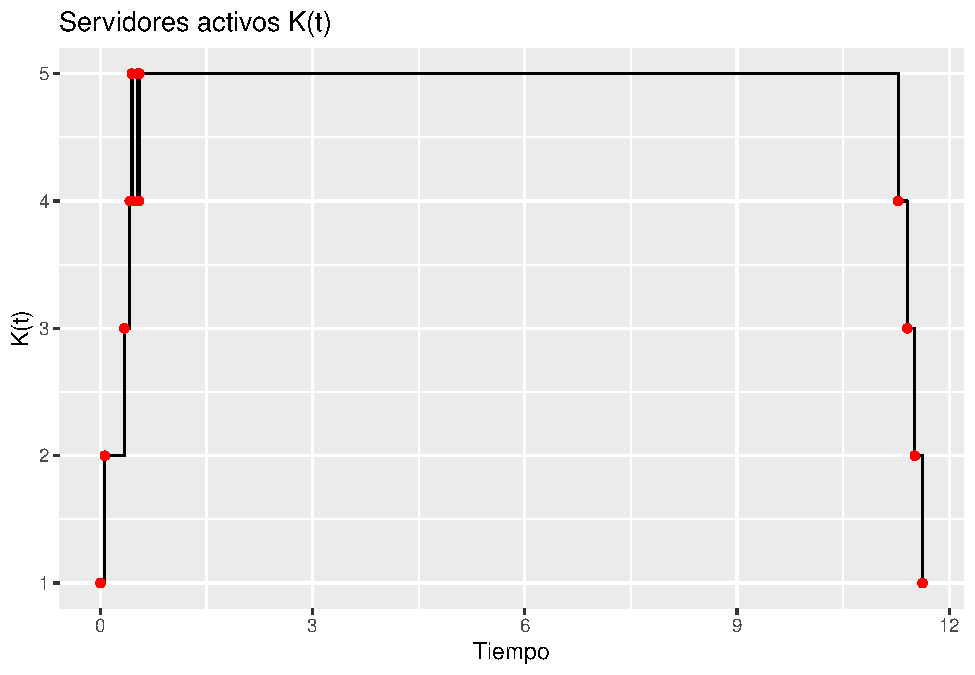
\includegraphics[width=350px,height=350px]{sistema_dinamico_files/figure-latex/unnamed-chunk-8-1} \end{center}

\subsection{Gráficos}\label{graficos-1}

\begin{flushright}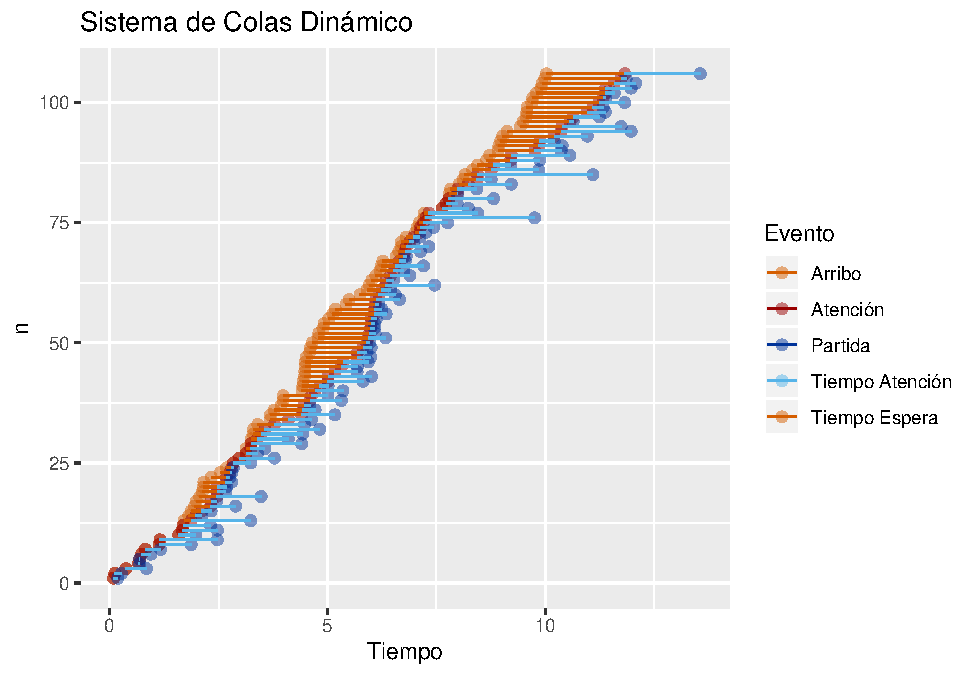
\includegraphics{sistema_dinamico_files/figure-latex/unnamed-chunk-9-1} \end{flushright}

\newpage

\section{Comparación del Rendimiento}\label{comparacion-del-rendimiento}

A fin de aclarar el comportamiento de estos dos sistemas, realizamos
\(N=500\) simulaciones de cada uno (manteniendo los mismos parámetros),
para luego tratar de estimar algunas caracteristicas de los sistemas
como por ejemplo el \textbf{Tiempo que los clientes estuvieron en
espera} y el \textbf{Tiempo de oscio de los Servidores}. A continuación
las comparaciones en cada criterio.

\subsubsection{Tiempo que los clientes estuvieron en
espera.}\label{tiempo-que-los-clientes-estuvieron-en-espera.}

Para estudiar el tiempo de espera mostramos una tabla que contiene una
parte de los resultados obtenidos en las simuaciones con cada modelo, y
además un histograma de los tiempos para cada modelo, que nos permitirá
comprender el comportamiento de la variable ``tiempo de espera del
cliente``.

\begin{center}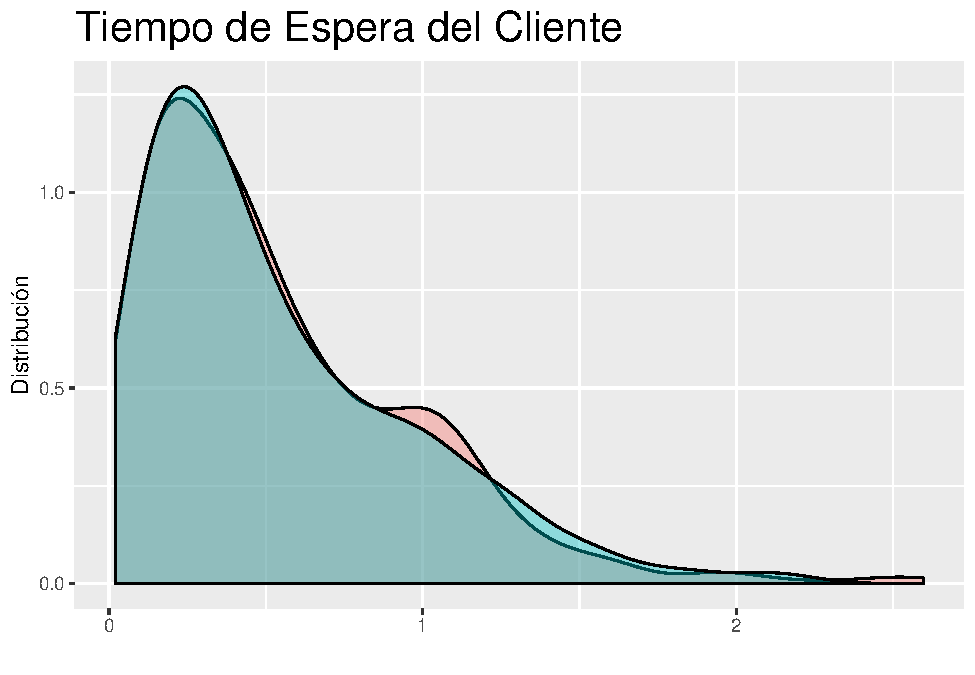
\includegraphics[width=280px,height=280px]{sistema_dinamico_files/figure-latex/unnamed-chunk-14-1} \end{center}

\begin{center}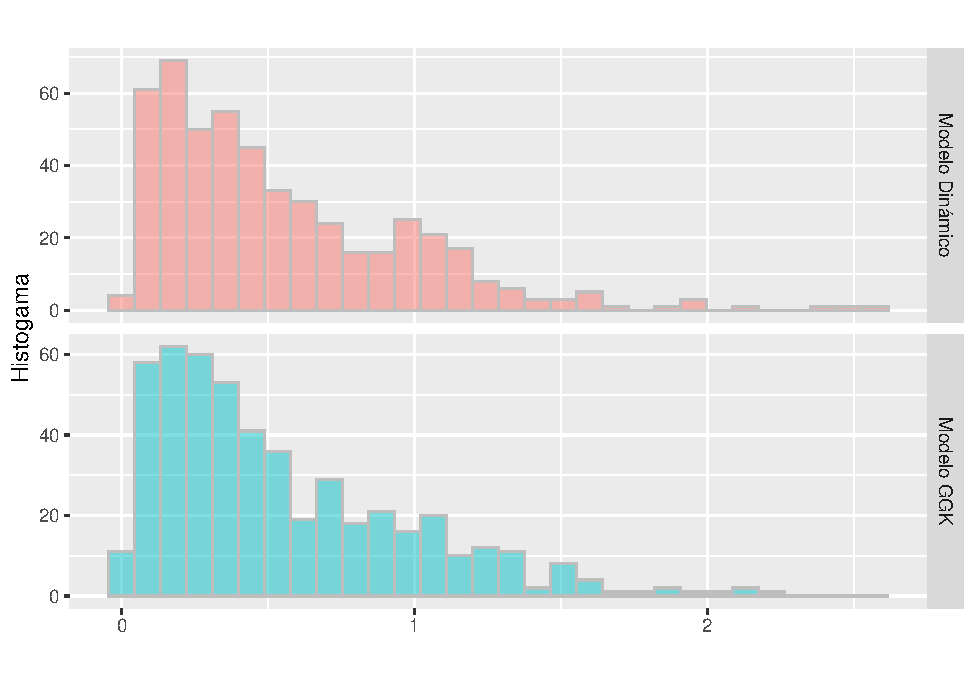
\includegraphics[width=280px,height=280px]{sistema_dinamico_files/figure-latex/unnamed-chunk-15-1} \end{center}

\begin{center}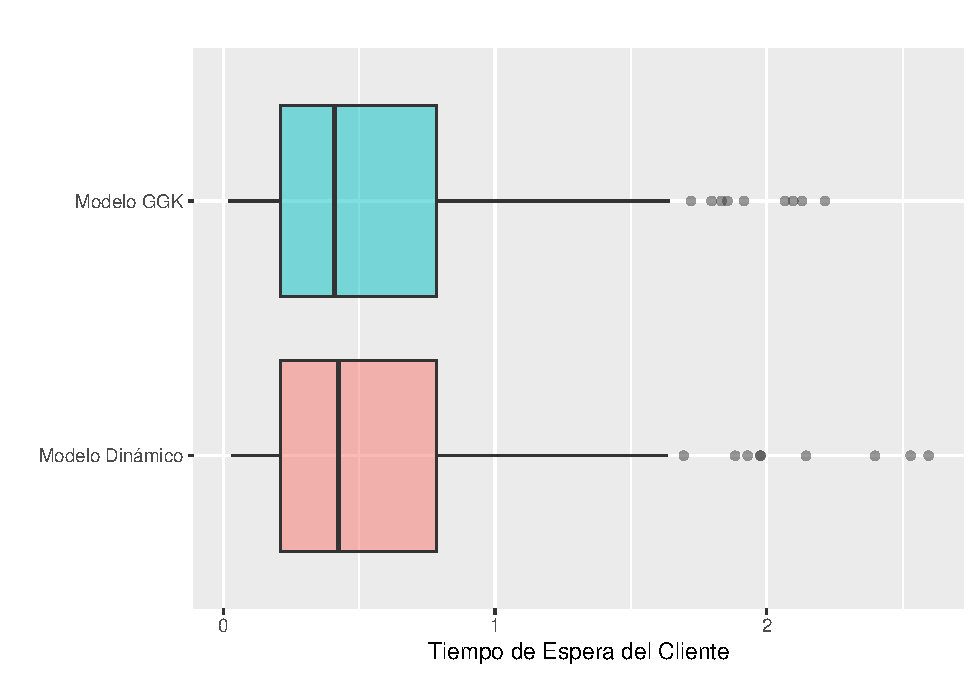
\includegraphics[width=280px,height=280px]{sistema_dinamico_files/figure-latex/unnamed-chunk-16-1} \end{center}

\newpage

\subsubsection{Tiempo de oscio de los
Servidores.}\label{tiempo-de-oscio-de-los-servidores.}

De igual manera con el objetivo de estudiar la variable ``tiempo de
oscio'' mostramos una tabla que contiene una parte de los resultados
obtenidos en las simuaciones con cada modelo, y además una gráfica de la
función de distribución aproximada de esta variable.

.

\begin{center}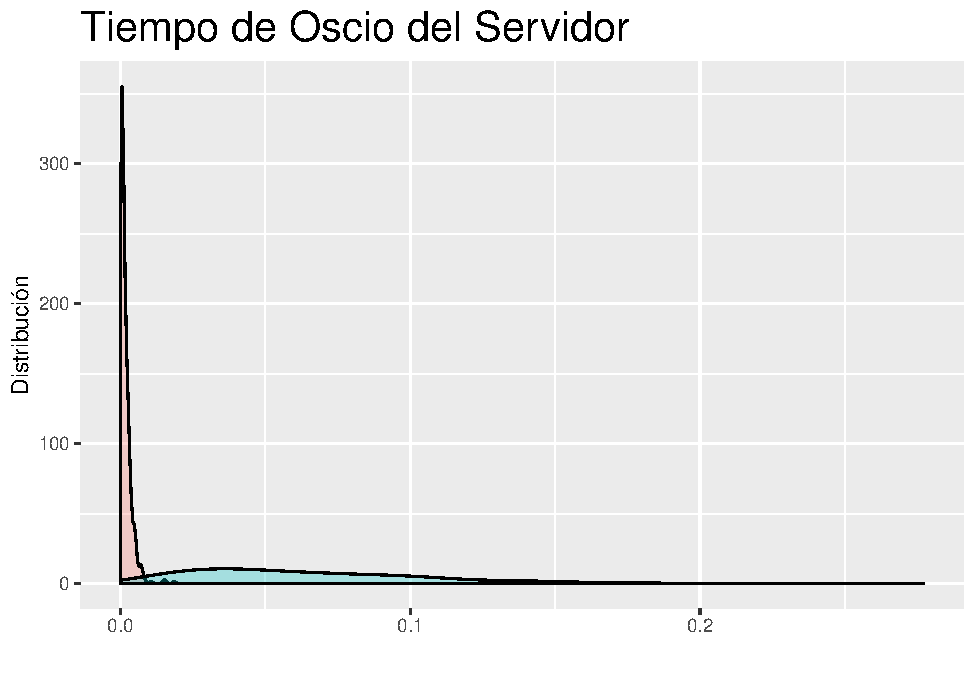
\includegraphics[width=280px,height=280px]{sistema_dinamico_files/figure-latex/unnamed-chunk-19-1} \end{center}

\begin{center}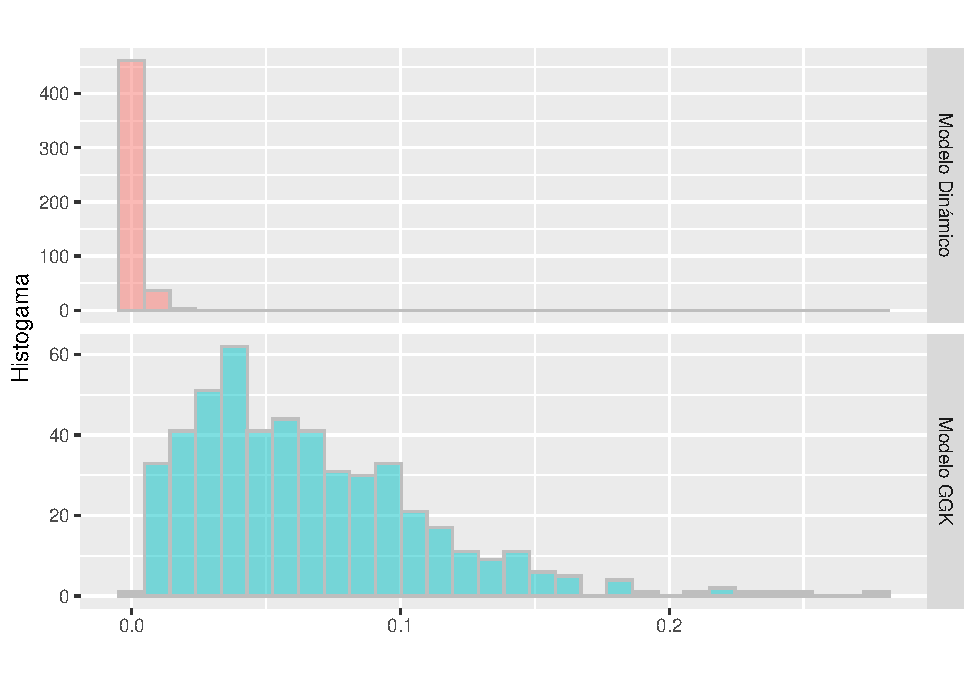
\includegraphics[width=280px,height=280px]{sistema_dinamico_files/figure-latex/unnamed-chunk-20-1} \end{center}

\begin{center}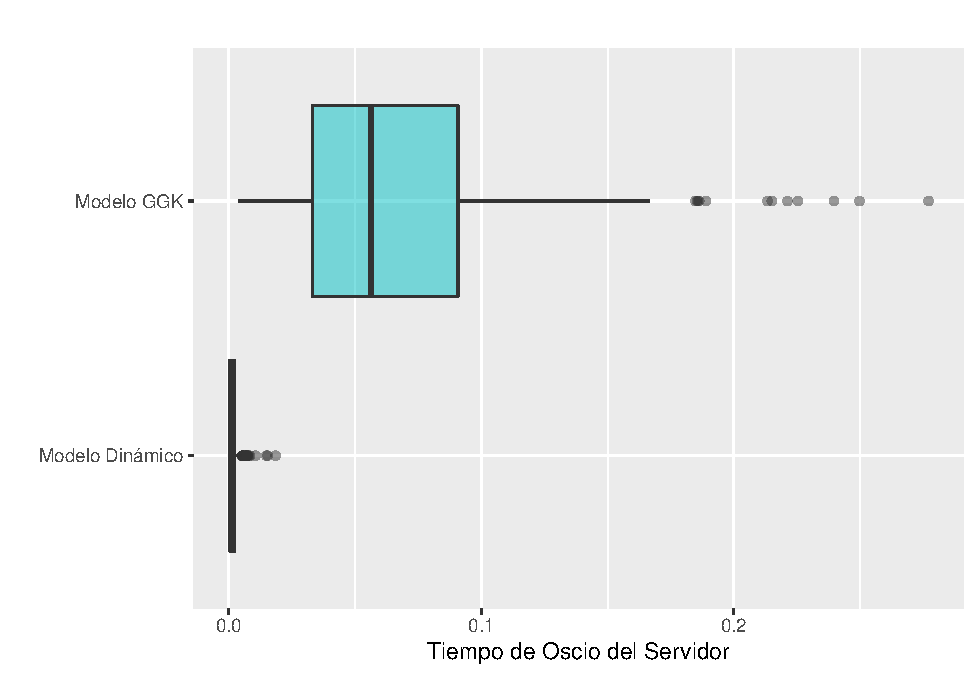
\includegraphics[width=280px,height=280px]{sistema_dinamico_files/figure-latex/unnamed-chunk-21-1} \end{center}

\newpage

\section{Conclusiónes}\label{conclusiones}

Partiendo de los datos obtenidos del punto anterior, podemos concluir lo
siguiente:

\begin{itemize}
\item
  Por una parte al analizar el ``Tiempo de espera del Cliente''"
  observamos que presenta un comportamiento muy similar en ambos
  modelos, esto se evidencia claramente en la enorme similitud de sus
  distribuciones. Esto era de esperarce ya que los tiempo de arribo de
  los clientes los tomamos con la misma distribución para ambos modelos.
\item
  En cuanto al ``Tiempo de Oscio de los servidores'', se ve una
  contundente diferencia entre los dos modelos, se ve de inmediato que
  el modelo dinámico es muchísimo más eficiente, es casi nulo en la
  mayoria de los casos. Esto debido a la politica que impusimos sobre la
  apertura y cierre de los servidores que evita precisamente el tiempo
  de oscio de los servidores, y que como vemos produce excelentes
  resultados de rendimiento. A diferencia del modelo estático, en donde
  se tienen tiempos de oscio de los servidores muchísimo más elevados.
\item
  De los dos puntos anteriores se puede concluir que el modelo dinámico
  presenta una importante mejora de rendimiento, es decir que al optar
  por una política de apertura y cierre de servidores se minimiza el
  costo relacionado al tiempo de oscio de los servidores, y además no
  afecta el rendimiento de los tiempos de espera de los clientes. Por lo
  tanto si se necesita escojer uno de los dos modelos (el estático, o el
  dinámico) se debe optar por el modelo dinámico por las razones antes
  expuestas.
\end{itemize}


\end{document}
